\chapter{Ideen und Konzepte}
\section{Grundkonzept}
% TODO Beschreibung wie das Problem im Ansatz gelöst werden soll
 Als Erstes wird die Usersimilarität und die Itemsimilarität im Featurespace, wie im Kapitel \ref{ch:StandDerPraxis} \nameref{ch:StandDerPraxis} beschrieben, berechnet. Dazu wird das Ähnlichkeitsmass Cosinus Similarität verwendet. Die Entscheidung die Cosinus Similarität und nicht die Pearson Korrelation zu verwenden wurde auf Grund der folgenden Nachteile der Pearson Korrelation getroffen:
\begin{itemize}
    \item Ein Nachteil der Pearson Korrelation ist, dass User mit wenigen Ratings eine hohe Ähnlichkeit aufweisen. (\cite{Ekstrand2011}).
    \item Die Person Korrelation wurde zur Berechnung der Item-Item Similarität vorgeschlagen, jedoch funktioniert die Pearson Korrelation schlechter als die Cosinus Similarität (\cite{10.1145/371920.372071}).
    
    
\end{itemize}

Des Weiteren wird die Principal Componant Analysis auf dem MovieLens 25M Dataset berechnet. Danach wird die Mahalanobisdistanz zwischen allen Datenpunkten auf dem transformierten Dataset berechnet. Dies wird mit dem Dataset mit allen Eigenvektoren, wie auch mit dem Dataset mit den Eigenvektoren, welche 90\% der Datenvarianz erklären, berechnet.

Als Nächstes werden die Top $N$ Nachbaren sowohl im Feature Space, als auch im Principal Component Space berechnet. Die Top $N$ Nachbaren werden dann miteinander verglichen. Die folgenden Abbildung \ref{fig:Komponentendiagramm} zeigt einen ersten Entwurf, wie die Software aufgebaut werden soll.

\begin{figure}[ht]
	\centering
	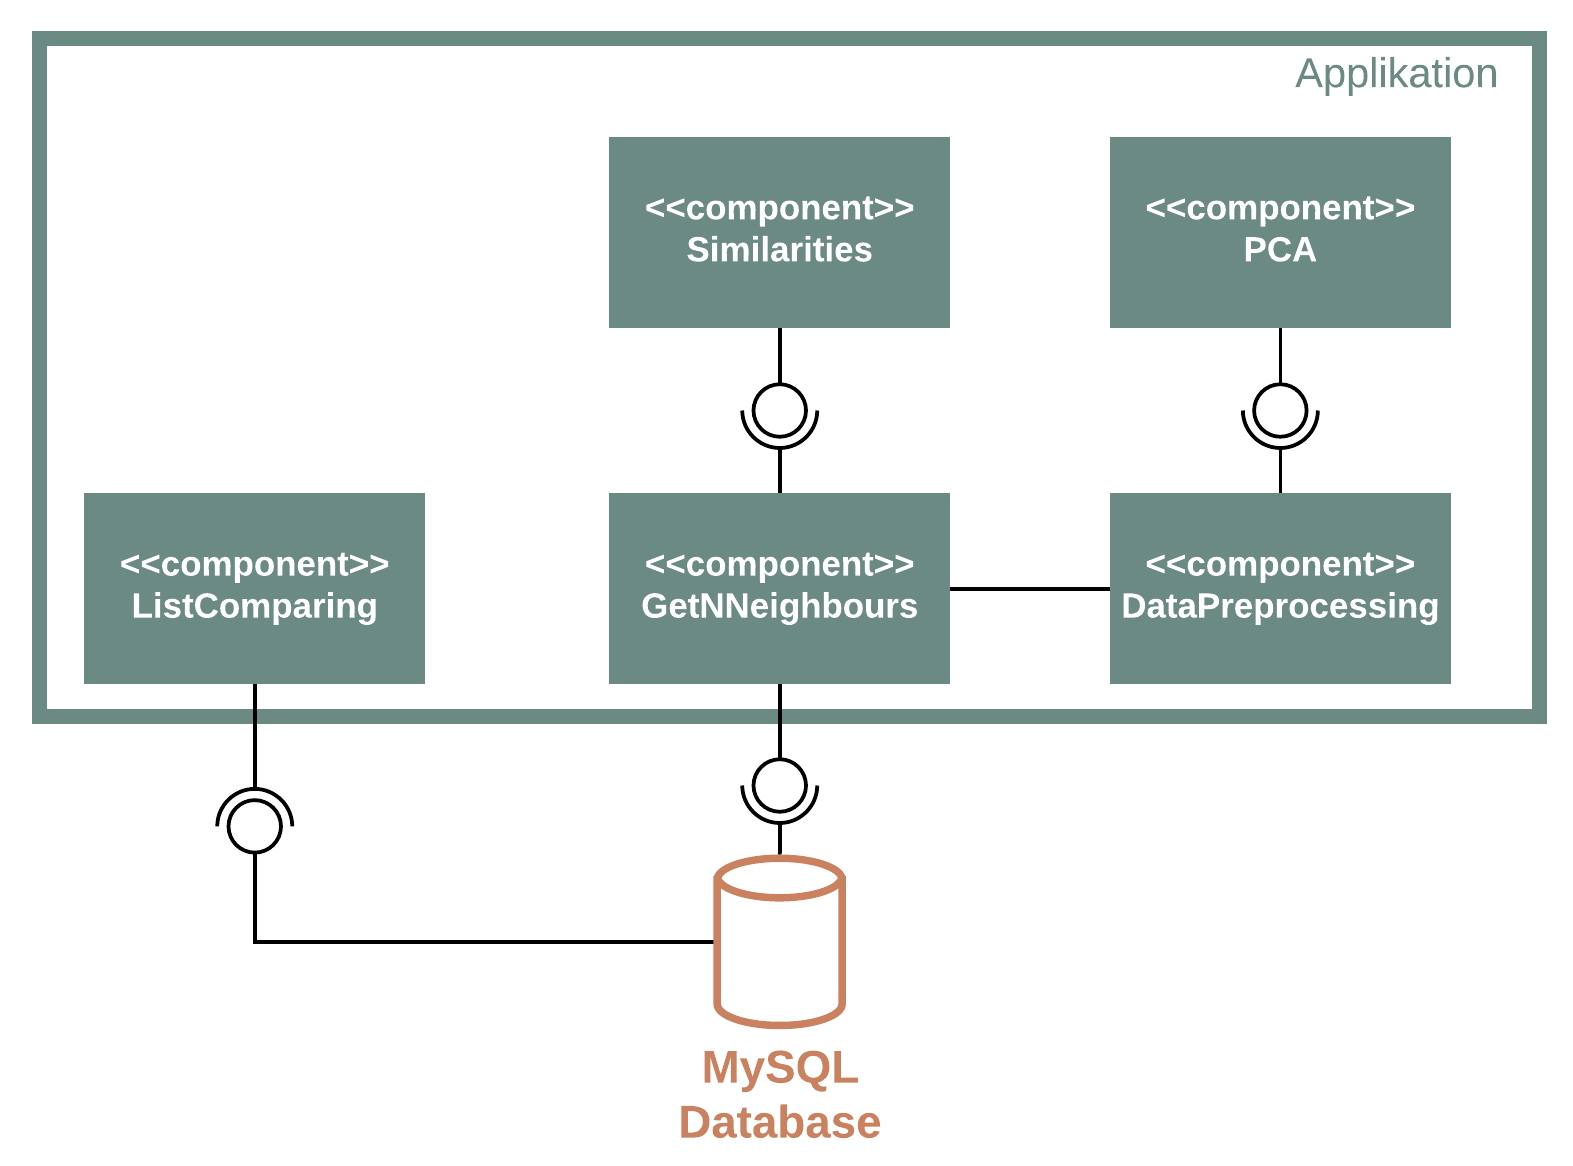
\includegraphics[keepaspectratio,width=0.66\linewidth]{img/Software Architektur BA.png}
	\caption{Komponentendiagramm}
	\label{fig:Komponentendiagramm}
\end{figure}

\newpage
\section{Testimplementationen}
Damit die einzelnen Komponenten funktionieren, wurden Prototypen implementiert und auf einem kleineren Trainingsset getestet.

\subsection{Data Preprocessing}
Um aus dem Movie Dataset, bestehend aus den Tripplets $(User, Item, Rating)$, eine Ratingmatrix $R$ zu kreieren, wird das Dataset mit folgender Funktion transformiert:

\begin{lstlisting}[language=Python, caption= Create Rating Matrix, label=lst:Create Rating Matrix]
import pandas as pd

def create_rating_matrix():
    Mean = movies.groupby(by="userId", as_index=False)['rating'].mean()
    Ratings = pd.pivot_table(movies,values='rating',index='movieId',columns='userId')
       
    # Replacing NaN by zero
    Ratings = Ratings.fillna(0)

    return Ratings        
\end{lstlisting}

\subsection{Principal Component Analysis}

Der erste Prototyp der Principal Component Analyse wurde mit der SciKit-learn\footnote{Library für Datenanalyse (\cite{scikit-learn}).} Implementation der Principal Component Analyse erstellt.

\begin{lstlisting}[language=Python, caption= Principal Component Analyse mit SciKit-learn,label=lst:PCA mit sci-kit]
from sklearn.preprocessing import StandardScaler
from sklearn.decomposition import PCA
from sklearn.preprocessing import RobustScaler

def compute_pca(Ratings):
    Ratings = create_rating_matrix()
    X = Ratings.values
    scaler = RobustScaler()
    X_tranformed = scaler.fit_transform(X)
    est = PCA(random_state=0).fit(X_tranformed)
    
    #Get Variance explained per PC
    v_ratio = est.explained_variance_ratio_
    
    #Creat Plot Showing Cumulative Sum of Variance per PC
    data = pd.DataFrame({'# of Features': range(1, len(v_ratio) + 1), '% Variance explained': np.cumsum(v_ratio * 100)})
    plt.plot(data)
    data.plot(x=0, y=1, grid=True, figsize=(10, 8))
    plt.show()
    
    return est

\end{lstlisting}

\noindent Trotz des kleinen Trainingsset, konnte die Principal Component Analyse mit dem SciKit-learn Prototypen \ref{lst:PCA mit sci-kit} nicht berechnet werden, da nicht genug Memory vorhanden war. Durch die Anforderung mit parallel laufenden Libraries zu arbeiten, wurde ein Prototyp mit Tensorflow \footnote{Tensorflow ist eine Open Source Machine Learning Plattform (\cite{tensorflow2015-whitepaper}).} erstellt.


\begin{lstlisting}[language=Python, caption= Principal Component Analyse mit Tensorflow, label=lst:PCA mit Tensorflow]
import tensorflow as tf
import tensorflow_transform as tft
import pandas as pd

def pca_tf():
    Ratings = create_rating_matrix()
    X = tf.constant(Ratings.values)
    X_normalized = normalize(X)
    PC= tft.pca(X_normalized,8)
    PC = PC.numpy()
    X_pca = pd.DataFrame(PC)
    
    return X_pca
    
def normalize(data):
    # creates a copy of data
    X = tf.identity(data)
    # calculates the mean
    X -= tf.reduce_mean(data, axis=0)
    return X

\end{lstlisting}

Ein Problem der Tensorflow Implementation der Principal Component Analyse ist, dass der Parameter \textit{Anzahl Dimensionen}, welche behalten werden möchten, mitgegeben werden muss. Laut Aufgabenstellung soll mit allen Eigenvektoren und mit den Eigenvektoren, welche 90\% der Varianz erklären, gerechnet werden. Die Anzahl benötigten Dimensionen, um 90\% der Varianz beizubehalten, kann jedoch erst nach der Principal Component Analyse berechnet werden. Deshalb wurde entschieden, die Principal Component Analyse selbst zu implementieren.

\subsection{Similarities}
Zur Berechnung der User- / Item-Similarität wurde ein Prototyp der Cosinus Similarität und der Mahalonobis Distanz erstellt.

\begin{lstlisting}[language=Python, caption= Cosinus Similarität, label=lst:Cosinus Similarität]
from sklearn.metrics.pairwise import cosine_similarity
import numpy as np
import pandas as pd

def _get_cosine_similarity(Ratings):
    cs = cosine_similarity(Ratings)
    np.fill_diagonal(cs, 0)
    cosine_similarity = pd.DataFrame(cs, index=Ratings.index)
    cosine_similarity.columns = Ratings.index
    
    return cosine_similarity

\end{lstlisting}

\begin{lstlisting}[language=Python, caption= Mahalanobis Distanz, label=lst:Mahalanobis Distanz]
from scipy.spatial import distance
import pandas as pd
import numpy as np
import tensorflow_probability as tfp

def _get_mahalanobis_distance(Ratings):

    Ratings = Ratings.values

    i=0
    mahalanobis_dist = []
    Cov = tfp.stats.covariance(Ratings).numpy()
    for i in range(len(Ratings)-1):
        j=0
        row_vec = []
        for j in range(len(Ratings)-1):
            dist= distance.mahalanobis(Ratings[i],Ratings[j],Cov)
            dist = dist.tolist()
            row_vec.append(dist)
            j+=1
        row_vec = row_vec.tolist()
        mahalanobis_dist.append(row_vec)
        i+=1
    np.fill_diagonal(mahalanobis_dist, 0)
    maha_dist = pd.DataFrame(mahalanobis_dist, index=Ratings.index)
    maha_dist.columns = Ratings.index
    return maha_dist
\end{lstlisting}